\documentclass[journal,12pt,twocolumn]{IEEEtran}

\usepackage{setspace}
\usepackage{gensymb}

\singlespacing


\usepackage[cmex10]{amsmath}

\usepackage{amsthm}

\usepackage{mathrsfs}
\usepackage{txfonts}
\usepackage{stfloats}
\usepackage{bm}
\usepackage{cite}
\usepackage{cases}
\usepackage{subfig}

\usepackage{longtable}
\usepackage{multirow}

\usepackage{enumitem}
\usepackage{mathtools}
\usepackage{steinmetz}
\usepackage{tikz}
\usepackage{circuitikz}
\usepackage{verbatim}
\usepackage{tfrupee}
\usepackage[breaklinks=true]{hyperref}
\usepackage{graphicx}
\usepackage{tkz-euclide}
\usepackage{float}

\usetikzlibrary{calc,math}
\usepackage{listings}
    \usepackage{color}                                            %%
    \usepackage{array}                                            %%
    \usepackage{longtable}                                        %%
    \usepackage{calc}                                             %%
    \usepackage{multirow}                                         %%
    \usepackage{hhline}                                           %%
    \usepackage{ifthen}                                           %%
    \usepackage{lscape}     
\usepackage{multicol}
\usepackage{chngcntr}

\DeclareMathOperator*{\Res}{Res}

\renewcommand\thesection{\arabic{section}}
\renewcommand\thesubsection{\thesection.\arabic{subsection}}
\renewcommand\thesubsubsection{\thesubsection.\arabic{subsubsection}}

\renewcommand\thesectiondis{\arabic{section}}
\renewcommand\thesubsectiondis{\thesectiondis.\arabic{subsection}}
\renewcommand\thesubsubsectiondis{\thesubsectiondis.\arabic{subsubsection}}


\hyphenation{op-tical net-works semi-conduc-tor}
\def\inputGnumericTable{}                                 %%

\lstset{
%language=C,
frame=single, 
breaklines=true,
columns=fullflexible
}
\begin{document}


\newtheorem{theorem}{Theorem}[section]
\newtheorem{problem}{Problem}
\newtheorem{proposition}{Proposition}[section]
\newtheorem{lemma}{Lemma}[section]
\newtheorem{corollary}[theorem]{Corollary}
\newtheorem{example}{Example}[section]
\newtheorem{definition}[problem]{Definition}

\newcommand{\BEQA}{\begin{eqnarray}}
\newcommand{\EEQA}{\end{eqnarray}}
\newcommand{\define}{\stackrel{\triangle}{=}}
\newcommand\hlight[1]{\tikz[overlay, remember picture,baseline=-\the\dimexpr\fontdimen22\textfont2\relax]\node[rectangle,fill=blue!50,rounded corners,fill opacity = 0.2,draw,thick,text opacity =1] {$#1$};}
\bibliographystyle{IEEEtran}
\providecommand{\mbf}{\mathbf}
\providecommand{\pr}[1]{\ensuremath{\Pr\left(#1\right)}}
\providecommand{\qfunc}[1]{\ensuremath{Q\left(#1\right)}}
\providecommand{\sbrak}[1]{\ensuremath{{}\left[#1\right]}}
\providecommand{\lsbrak}[1]{\ensuremath{{}\left[#1\right.}}
\providecommand{\rsbrak}[1]{\ensuremath{{}\left.#1\right]}}
\providecommand{\brak}[1]{\ensuremath{\left(#1\right)}}
\providecommand{\lbrak}[1]{\ensuremath{\left(#1\right.}}
\providecommand{\rbrak}[1]{\ensuremath{\left.#1\right)}}
\providecommand{\cbrak}[1]{\ensuremath{\left\{#1\right\}}}
\providecommand{\lcbrak}[1]{\ensuremath{\left\{#1\right.}}
\providecommand{\rcbrak}[1]{\ensuremath{\left.#1\right\}}}
\theoremstyle{remark}
\newtheorem{rem}{Remark}
\newcommand{\sgn}{\mathop{\mathrm{sgn}}}
\providecommand{\abs}[1]{\left\vert#1\right\vert}
\providecommand{\res}[1]{\Res\displaylimits_{#1}} 
\providecommand{\norm}[1]{$\left\lVert#1\right\rVert$}
%\providecommand{\norm}[1]{\lVert#1\rVert}
\providecommand{\mtx}[1]{\mathbf{#1}}
\providecommand{\mean}[1]{E\left[ #1 \right]}
\providecommand{\fourier}{\overset{\mathcal{F}}{ \rightleftharpoons}}
%\providecommand{\hilbert}{\overset{\mathcal{H}}{ \rightleftharpoons}}
\providecommand{\system}{\overset{\mathcal{H}}{ \longleftrightarrow}}
	%\newcommand{\solution}[2]{\textbf{Solution:}{#1}}
\newcommand{\solution}{\noindent \textbf{Solution: }}
\newcommand{\cosec}{\,\text{cosec}\,}
\providecommand{\dec}[2]{\ensuremath{\overset{#1}{\underset{#2}{\gtrless}}}}
\newcommand{\myvec}[1]{\ensuremath{\begin{pmatrix}#1\end{pmatrix}}}
\newcommand{\mydet}[1]{\ensuremath{\begin{vmatrix}#1\end{vmatrix}}}
\numberwithin{equation}{subsection}
\makeatletter
\@addtoreset{figure}{problem}
\makeatother
\let\StandardTheFigure\thefigure
\let\vec\mathbf
\renewcommand{\thefigure}{\theproblem}
\def\putbox#1#2#3{\makebox[0in][l]{\makebox[#1][l]{}\raisebox{\baselineskip}[0in][0in]{\raisebox{#2}[0in][0in]{#3}}}}
     \def\rightbox#1{\makebox[0in][r]{#1}}
     \def\centbox#1{\makebox[0in]{#1}}
     \def\topbox#1{\raisebox{-\baselineskip}[0in][0in]{#1}}
     \def\midbox#1{\raisebox{-0.5\baselineskip}[0in][0in]{#1}}
\vspace{3cm}
\title{Assignment No.1}
\author{RajaSekhar Jala}
\maketitle
\newpage
\bigskip
\renewcommand{\thefigure}{\theenumi}
\renewcommand{\thetable}{\theenumi}
Download all python codes from 
\begin{lstlisting}
https://github.com/Sekharjala/Assignments/blob/main/code
\end{lstlisting}
%
and pdf from 
%
\begin{lstlisting}
https://github.com/Sekharjala/Assignments/blob/main/Assignment1.pdf
\end{lstlisting}
%
\section{Question No.Matrices 1.76.1}
Question :
Find equation of line joining (1,2) and
(3,6) using determinants.
\section{Solution}
To construct a line joining $\Vec{A}=\myvec{1\\2}$ and $\vec{B}=\myvec{3\\6}$ ,let $\vec{n}$ be the normal vector then

\begin {align}
\vec{n^T} \vec {A}=c \label{eq:1} \\
\vec{n^T} \vec {B}=c  \label{eq:2} 
\end{align}
from Equations \eqref{eq:1} and \eqref{eq:2} \\
\begin{align}
    \vec{A}^T \vec {n}=c \\
    \vec{B}^T \vec {n}=c  \\
    \myvec{\vec{A}^T \\ \vec{B}^T} \vec{n}=\myvec{c \\ c} \\
    \myvec{1 &2 \\ 3&6} \vec{n}=\myvec{c\\c}
\end{align}
Augmented Matrix is 
\begin{align}
    \myvec{1&2&c\\3&6&c} \\
    \myvec{ 1 &  2 & c \\ 3&  6& c } \overset{3R_1-R_2\rightarrow R_2}{\longrightarrow} \myvec{ 1 &  2& c\\0 &  0 & -2c }
\end{align}
Thus, from the above row reduced form we can conclude that the given system of lines has solution iff c $\equiv$ 0 and points are collinear.
\begin{align}
    \myvec{ 1 &  2& 0\\0 &  0 & 0 } \\
    \myvec{1&2}\vec{n}=0
\end{align}
The normal vector $\vec{n}$ to a line is  orthogonal to the direction vector m then \\
\begin{align}
    \vec{m}^T\vec{n}=0
\end{align}
    Directional vector is 
\begin{align}
    \vec{m} = \myvec{1 \\ 2}
\end{align}
    Normal vector 
\begin{align}
    \vec{n}= \myvec{-2\\1}
\end{align}
    Equation of straight line is 
\begin{align}
    \myvec{-2&1} \vec{x}=0 
    %\begin{pmatrix} 1 &  2 \\ 0 &  0\end{pmatrix}  \vec{n}=\myvec{0\\0} \\
   % \vec{n}=\myvec{1&2 \\0&0}^{-1}  \myvec{0\\0} =\myvec{0\\0}
\end{align}
\begin{figure}[H]
\centering
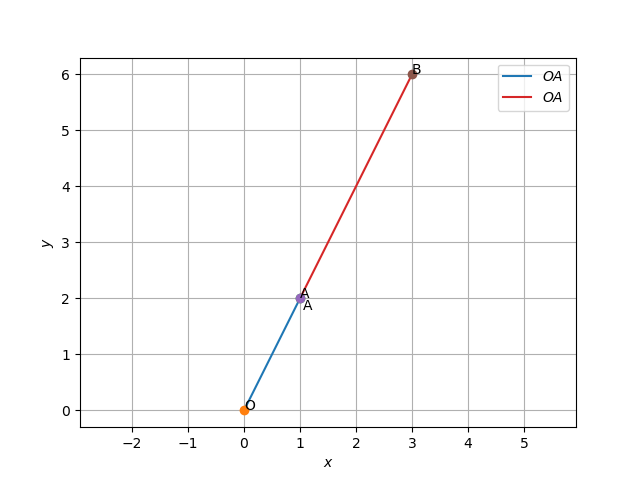
\includegraphics[width=\columnwidth]{Figure_1.png}
\caption{line formed with points \myvec{1&2} and \myvec{3&6} using Python}
\label{fig:1}
\end{figure}
\end{document}
